\subsection{Task 3: Weakly Connected Component}
In this experiment, we run weakly connected component in several datasets of various size.

\subsubsection{Plot}
We draw size-frequency plot in log-log scales.
\begin{figure}[h]
\begin{center}
     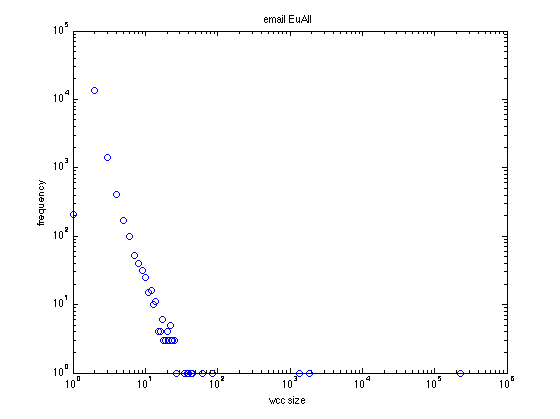
\includegraphics[width=0.8\textwidth]{FIG/t3_email_euall.png} 
\caption{Email-EuAll }
\label{t3:1}
\end{center}
\end{figure}

\begin{figure}[h]
\begin{center}
\begin{tabular}{cc}
     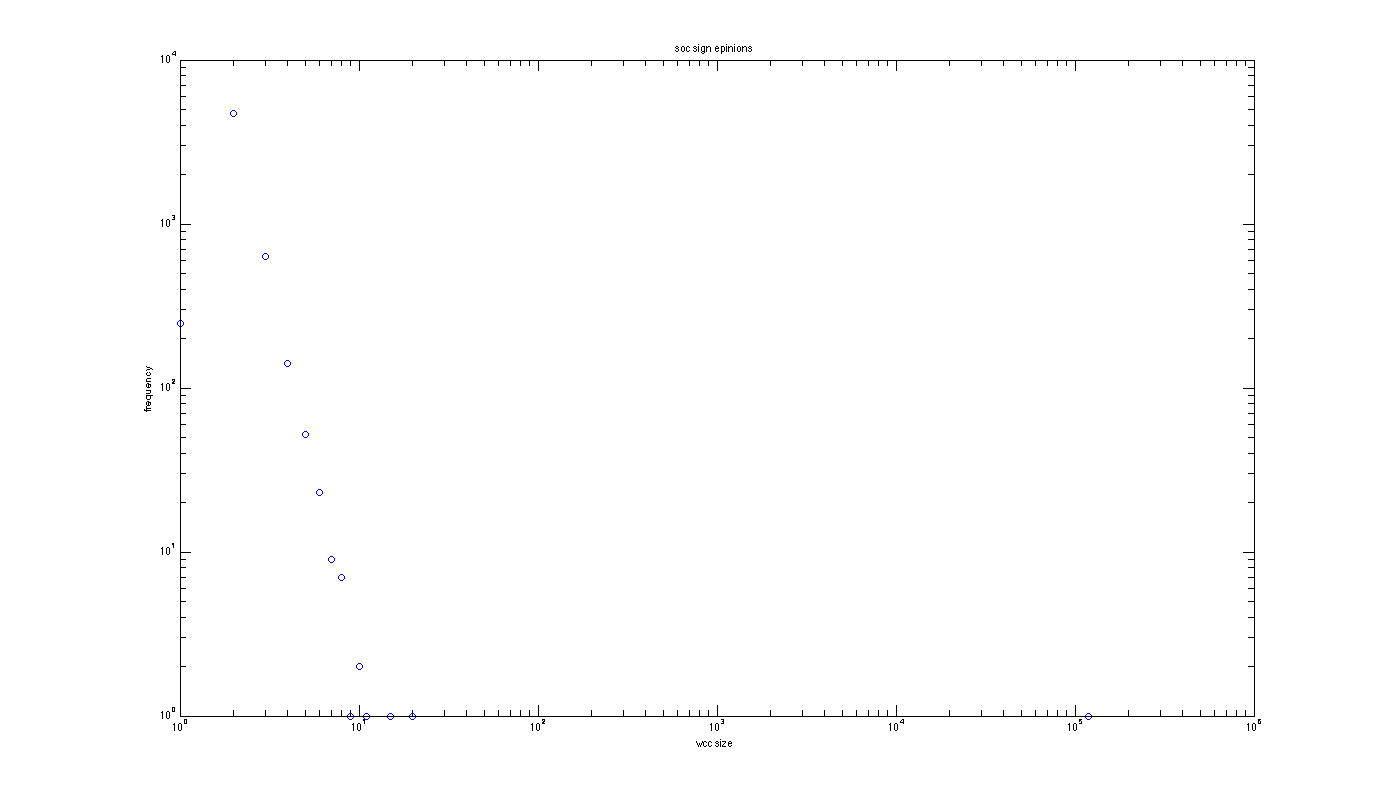
\includegraphics[width=0.8\textwidth]{FIG/t3_soc_sign_epinions.png} 
\end{tabular}
\caption{Soc-Sign-Epinions}
\label{t3:2}
\end{center}
\end{figure}


\begin{figure}[h]
\begin{center}
     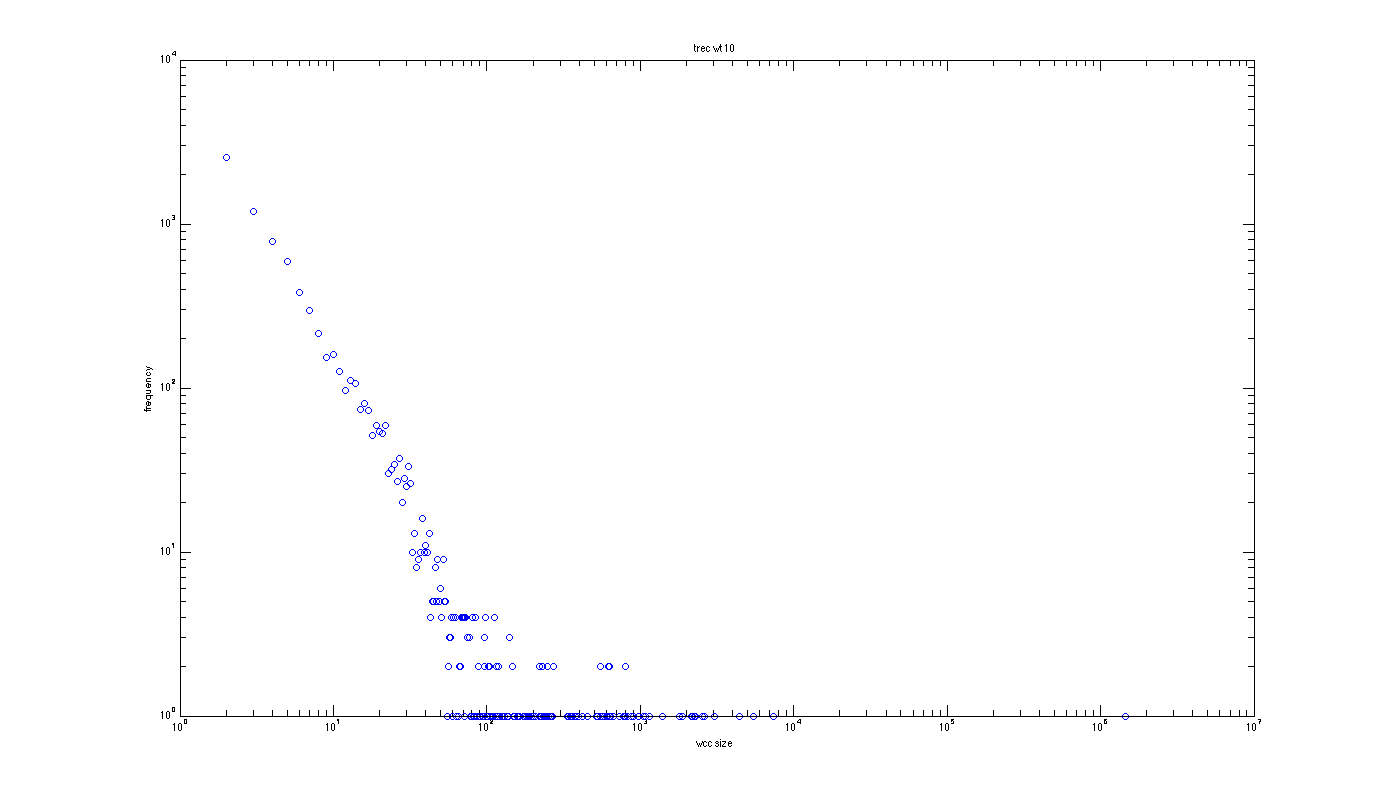
\includegraphics[width=0.8\textwidth]{FIG/t3_trec_wt10.png} 
\caption{Trec-wt10g}
\label{t3:3}
\end{center}
\end{figure}


\begin{figure}[h]
\begin{center}
     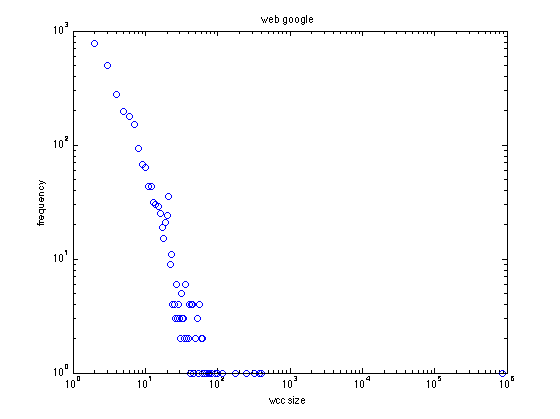
\includegraphics[width=0.8\textwidth]{FIG/t3_web_google.png} 
\caption{Google Web Graph}
\label{t3:4}
\end{center}
\end{figure}


\begin{figure}[h]
\begin{center}
     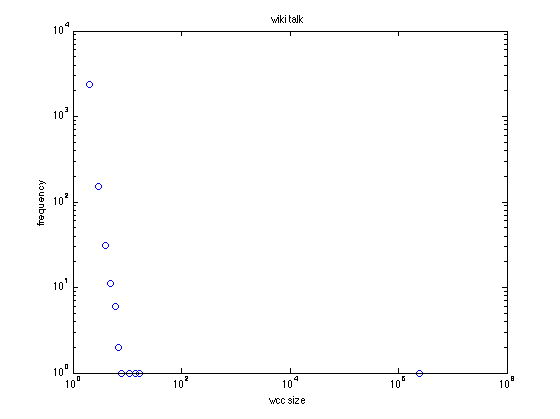
\includegraphics[width=0.8\textwidth]{FIG/t3_wiki_talk.png} 
\caption{Wiki Talk}
\label{t3:5}
\end{center}
\end{figure}

\subsubsection{Observation}
1. From the log-log scale frequency-size plot, we find that generally frequency-size follows the power law. Connected components of small sizes tend to occur more often those of larger sizes.

2. In all the plots, there is a giant connected component that contains the majority of nodes in the graph. 




